\documentclass[tikz]{standalone}
\usetikzlibrary{positioning}

\newcommand{\po}[2]{\draw [->, thick] (#1) to node[above] {\Large{so}} (#2);}
%\newcommand{\povis}[2]{\draw [->, thick] (#1) to node[above] {\Large{so}$,$ \Large{vis}} (#2);}
\newcommand{\povis}[2]{\draw [->, thick] (#1) to node[above] {\Large{so}} node[below] {\Large{vis}} (#2);}
\newcommand{\vis}[2]{\draw [->, thick, dashed] (#1) to node[above, sloped, near end] {\Large{vis}} (#2);}
\newcommand{\ar}[2]{\draw [->, thick, dotted] (#1) to node[above, sloped] {\Large{ar}} (#2);}
\newcommand{\vvis}[2]{\draw [->, thick, dashed, allow upside down] (#1) to node[above, sloped] {\Large{vis}} (#2);}

\begin{document}
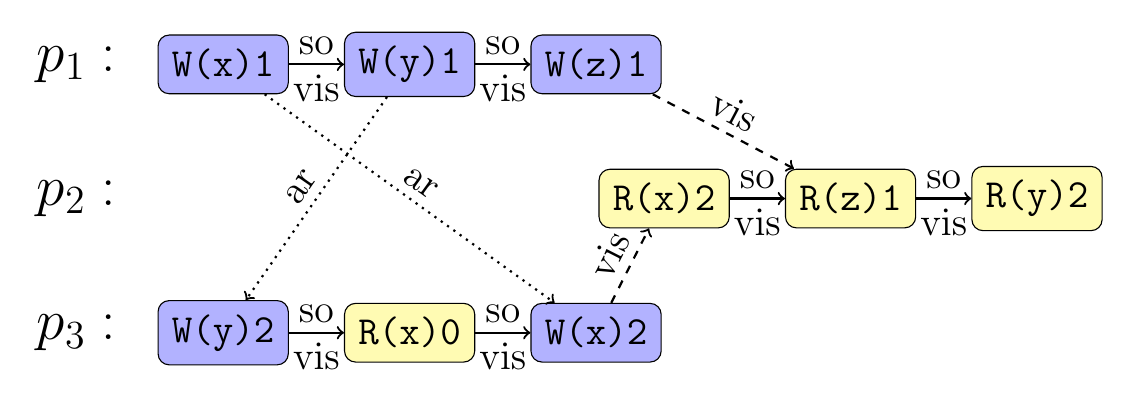
\begin{tikzpicture}
\tikzset{
  wop/.style = {rectangle, rounded corners, fill = blue!30, draw, font = \Large, inner sep = 5pt},
  rop/.style = {rectangle, rounded corners, fill = yellow!30, draw, font = \Large, inner sep = 5pt},
  process/.style = {font = \huge},
%  po/.style = {->, very thick},
%  rw/.style = {->, shorten >= 3pt, very thick, dashed},
%  vis/.style = {->, shorten >= 3pt, very thick, dashed}
}

  \node (p1) [process] {$p_1:$};
  \node (wx1) [wop, right = 0.4cm of p1] {\texttt{W(x)1}};
  \node (wy1) [wop, right = 0.7cm of wx1] {\texttt{W(y)1}};
  \node (wz1) [wop, right = 0.7cm of wy1] {\texttt{W(z)1}};

  \node (p2) [process, below = 1.0cm of p1] {$p_2:$};
  \node (rx2) [rop, right = 6cm of p2] {\texttt{R(x)2}};
  \node (rz1) [rop, right = 0.7cm of rx2] {\texttt{R(z)1}};
  \node (ry2) [rop, right = 0.7cm of rz1] {\texttt{R(y)2}};

  \node (p3) [process, below = 1.0cm of p2] {$p_3:$};
  \node (wy2) [wop, right = 0.4cm of p3] {\texttt{W(y)2}};
  \node (rx0) [rop, right = 0.7cm of wy2] {\texttt{R(x)0}};
  \node (wx2) [wop, right = 0.7cm of rx0] {\texttt{W(x)2}};

  \povis{wx1}{wy1};
  \povis{wy1}{wz1};

  \povis{rx2}{rz1};
  \povis{rz1}{ry2};

  \povis{wy2}{rx0};
  \povis{rx0}{wx2};

  \vvis{wx2}{rx2};
  \vvis{wz1}{rz1};

  \ar{wy1}{wy2};
  \ar{wx1}{wx2}
\end{tikzpicture}
\end{document}
